\documentclass[12pt]{article}
\usepackage[margin=2cm]{geometry}

\usepackage{graphicx}
\usepackage{float}

\usepackage{xeCJK}
\setmainfont{Times New Roman}
\setCJKmainfont[AutoFakeBold=true,AutoFakeSlant=true]{TW-Kai}
\renewcommand\contentsname{目錄}
\renewcommand\listfigurename{圖目錄}
\renewcommand\listtablename{表目錄}
\renewcommand\abstractname{摘要}
\renewcommand\figurename{圖}
\renewcommand\tablename{表}
\renewcommand\refname{參考文獻}

\usepackage{indentfirst}
\setlength{\parindent}{0em}
\setlength{\parskip}{0.5em}

\usepackage[hidelinks]{hyperref}
\newcommand*{\fullref}[1]{\hyperref[{#1}]{\ref*{#1} \nameref*{#1}}}

\renewcommand{\figureautorefname}{圖}
\renewcommand\tableautorefname{表}

\begin{document}

\title{Logic Synthesis and Verification PA2}
\author{B11107051 李品翰}
\date{}
\maketitle

\section{實驗環境與控制變因}

本報告中所有的模型訓練皆遵循 DeepGate2 的兩階段訓練策略，並設定以下控制變因：

\begin{itemize}
  \item Hidden Layer Dimensions: 64
  \item 一個階段 epoch 數: 20
  \item Batch Size: 64
  \item Learning Rate 衰減點 (\texttt{lr\_step}): 第 15 個 epoch
  \item 第一階段 loss weight: \texttt{W\_prob} = 1, \texttt{W\_rc} = 0, \texttt{W\_func} = 0
  \item 第二階段 loss weight: \texttt{W\_prob} = 3, \texttt{W\_rc} = 1, \texttt{W\_func} = 2
\end{itemize}

其餘未提及的參數皆與預設相同。下方實驗皆為改變其中的某個變因而產生的結果。

\section{Assignment 1: Hidden Layer Dimensions 對模型效能之影響}

本章節比較了 Hidden Layer Dimensions 在 32、64 與 128 時，模型對於 Truth Table distance prediction 與 Signal probability estimation 兩項任務上的表現。

\begin{figure}[H]
  \centering
  \caption{不同 Hidden Layer Dimensions 之 Total Loss 比較}
  \label{fig:n_dim_loss_compare}
  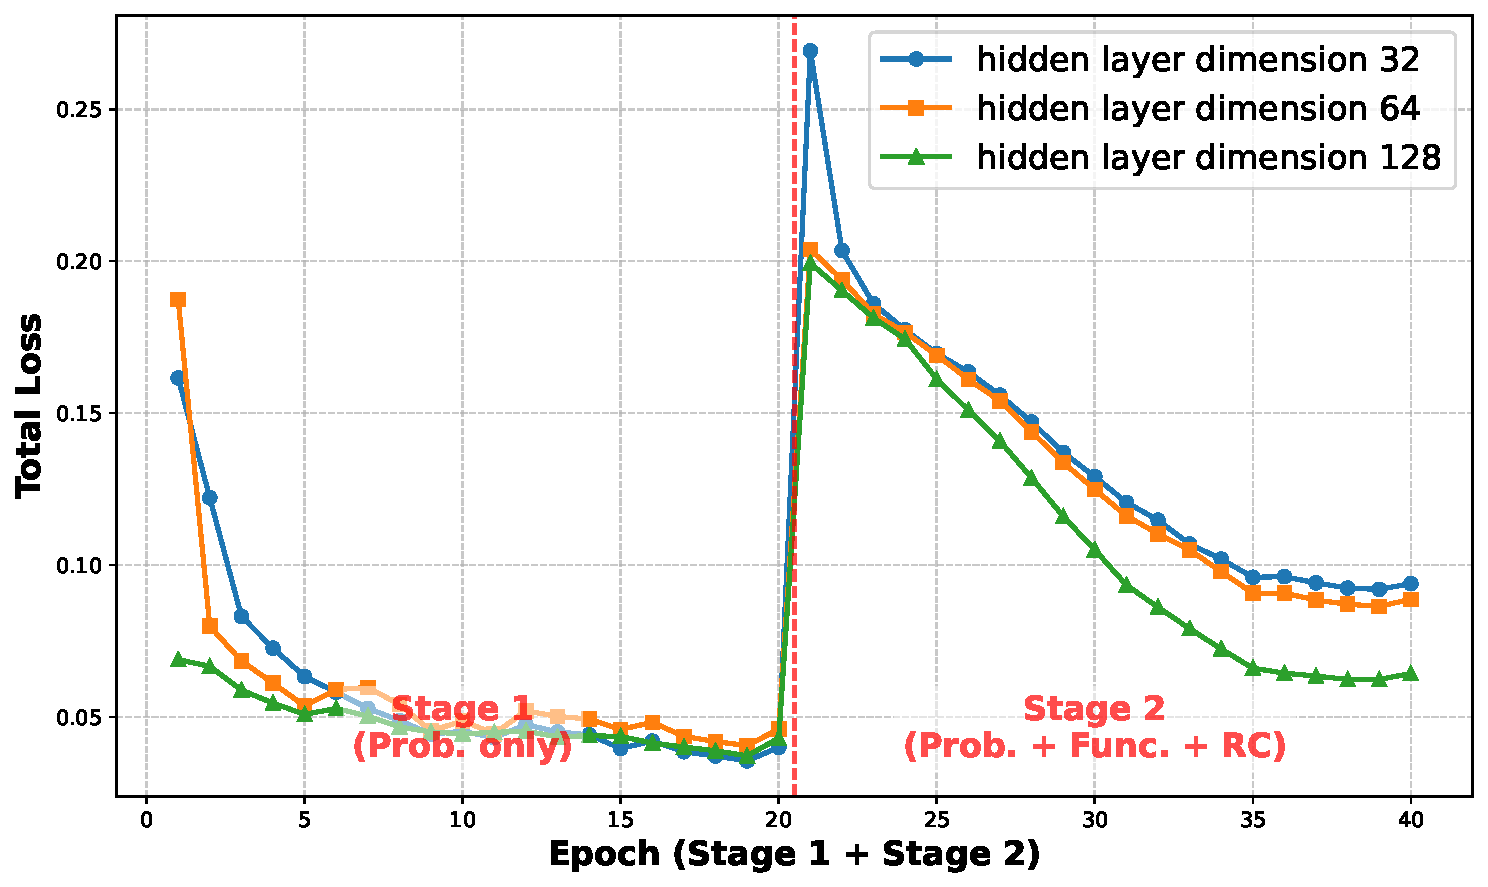
\includegraphics[width=0.7\linewidth]{n_dim_loss_compare.pdf}
\end{figure}

\begin{itemize}
  \begin{figure}[H]
    \centering
    \caption{不同 Hidden Layer Dimensions 之 Accuracy 比較}
    \label{fig:n_dim_accuracy_compare}
    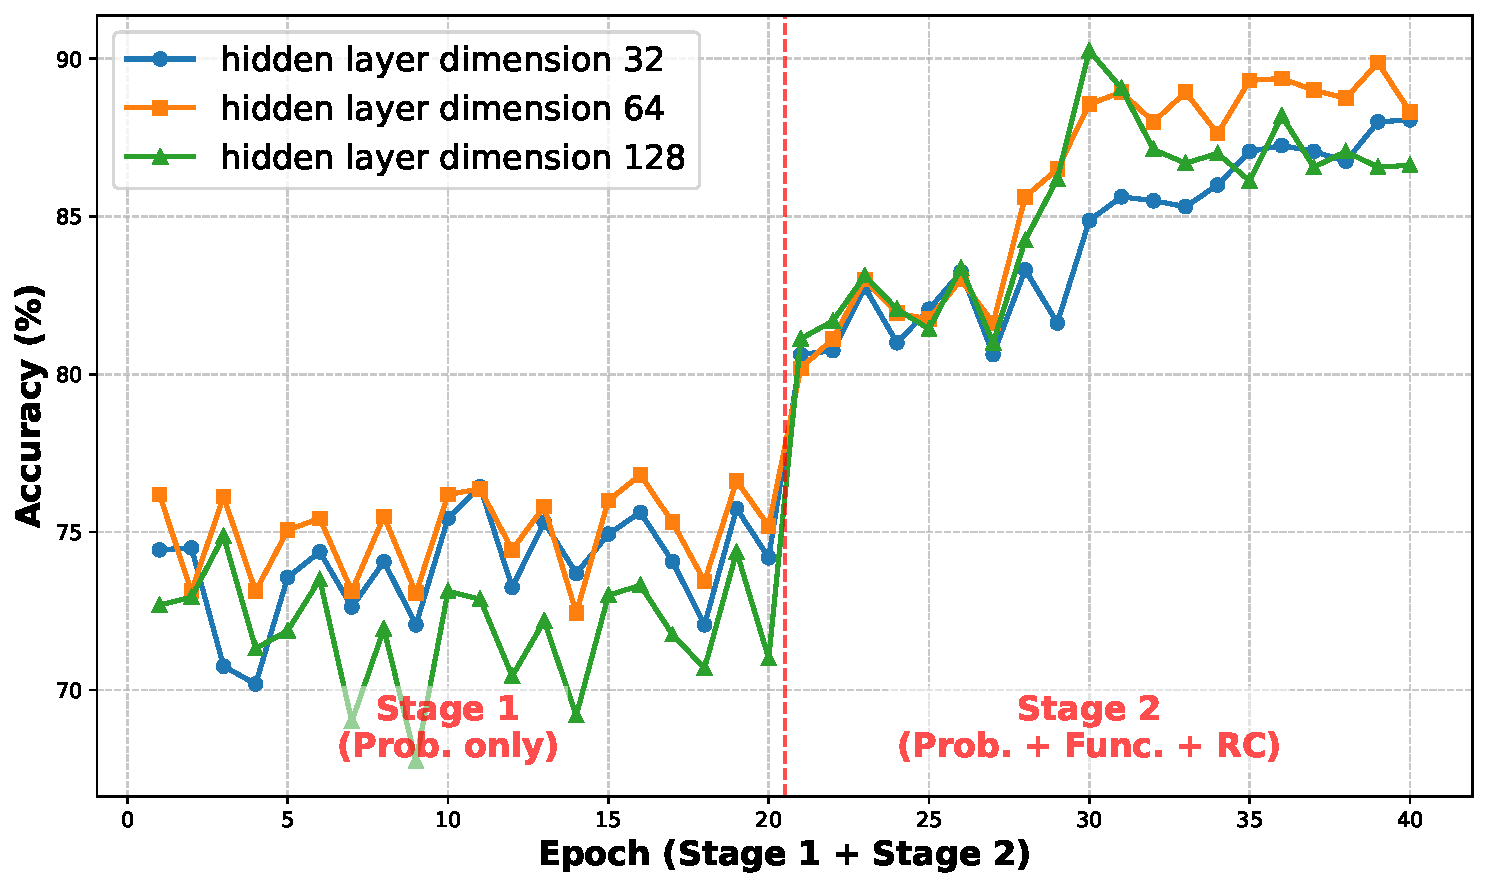
\includegraphics[width=0.7\linewidth]{n_dim_accuracy_compare.pdf}
  \end{figure}
  
  \begin{figure}[H]
    \centering
    \caption{不同 Hidden Layer Dimensions 之 LFunc 比較}
    \label{fig:n_dim_lfunc_compare}
    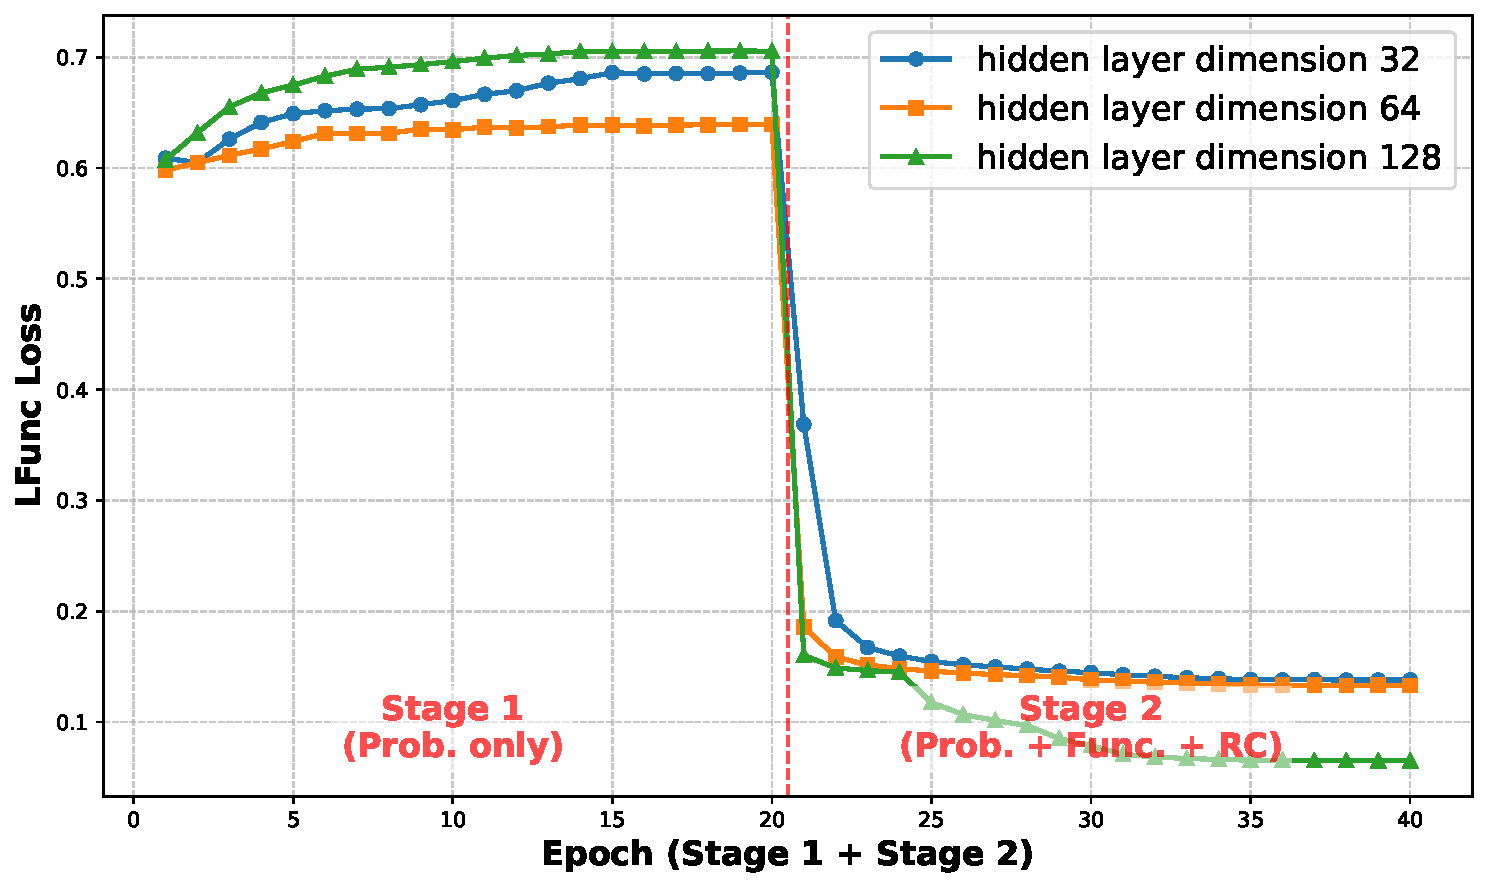
\includegraphics[width=0.7\linewidth]{n_dim_lfunc_compare.pdf}
  \end{figure}

  \item Truth Table distance prediction (LFunc 與 Accuracy)：
  如果同時看 \autoref{fig:n_dim_lfunc_compare} LFunc 和 \autoref{fig:n_dim_accuracy_compare} Accuracy 的曲線，會發現一個有趣的現象。在預測真值表誤差的 LFunc Loss 方面，Dim=128 的表現最好，能把誤差壓到最低 (大約 0.06)。但是在看最終分類是否正確的 Accuracy 時，反而是 Dim=64 拿到最高的準確率，Dim=128 的準確率反而稍微往下掉了。這表示 128 維雖然因為參數很多，可以把誤差算得非常精準，但可能有點鑽牛角尖 (也就是稍微過擬合了局部的特徵)，導致它在判斷界線 (Decision Boundary) 時反而容易出錯，失去了舉一反三的泛化能力 (Generalization)。整體看下來，Dim=64 是特徵學習與泛化能力平衡得最好的一個設定。

  \begin{figure}[H]
    \centering
    \caption{不同 Hidden Layer Dimensions 之 LProb 比較}
    \label{fig:n_dim_lprob_compare}
    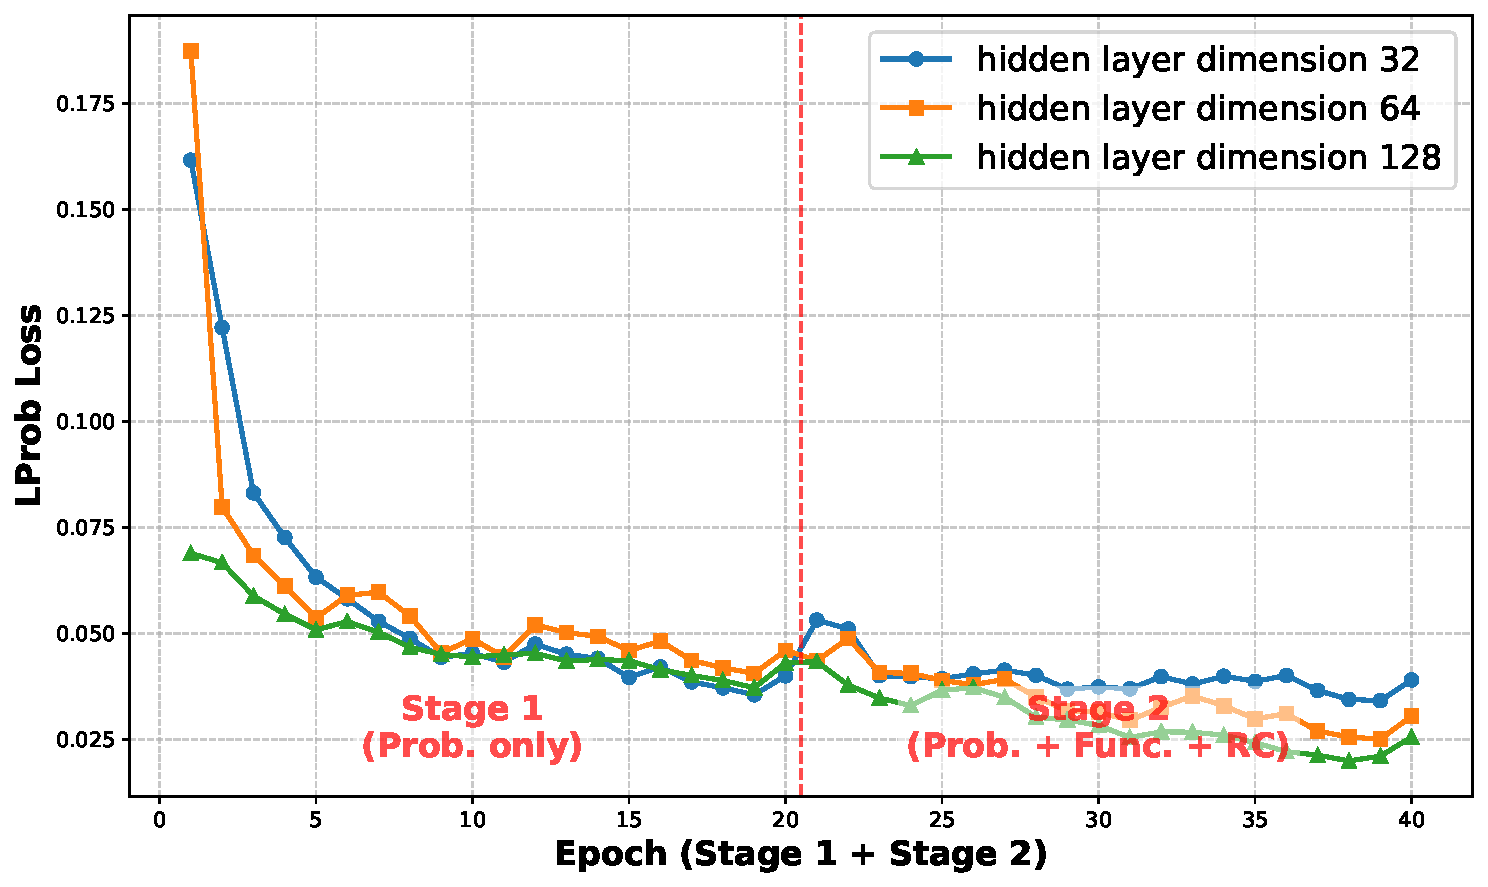
\includegraphics[width=0.7\linewidth]{n_dim_lprob_compare.pdf}
  \end{figure}
  
  \item Signal probability estimation (LProb)：
  從 \autoref{fig:n_dim_lprob_compare} LProb 曲線可以看出，進入 Stage 2 後，三個維度的模型都有穩定下降並收斂。其中 Dim=128 和 Dim=64 的最終結果相近 (約降到 0.025)，且都比 Dim=32 還要好。這代表 64 維已經有足夠的學習能力來抓到邏輯閘的機率特徵，就算把維度繼續加大到 128，帶來的幫助也非常小。
\end{itemize}

\section{Assignment 2: Ablation Study}

本章節透過移除 Pairwise TT Loss 以及 Orthogonal PI Initialization 這兩項機制的 Ablation Study，來驗證其對模型效能的實質貢獻。

\subsection{Pairwise TT Loss 之有效性}

DeepGate2 引入 Pairwise TT Loss 主要為了解決 NOT gate problem，即邏輯閘與其反相器在結構與機率上高度相似，但功能完全相反的情境。本實驗將第二階段的 \texttt{W\_func} 權重強制設為 0 來觀察其影響。

\begin{itemize}
  \begin{figure}[H]
    \centering
    \caption{開關 Pairwise TT Loss 之 LFunc 比較}
    \label{fig:no_tt_lfunc}
    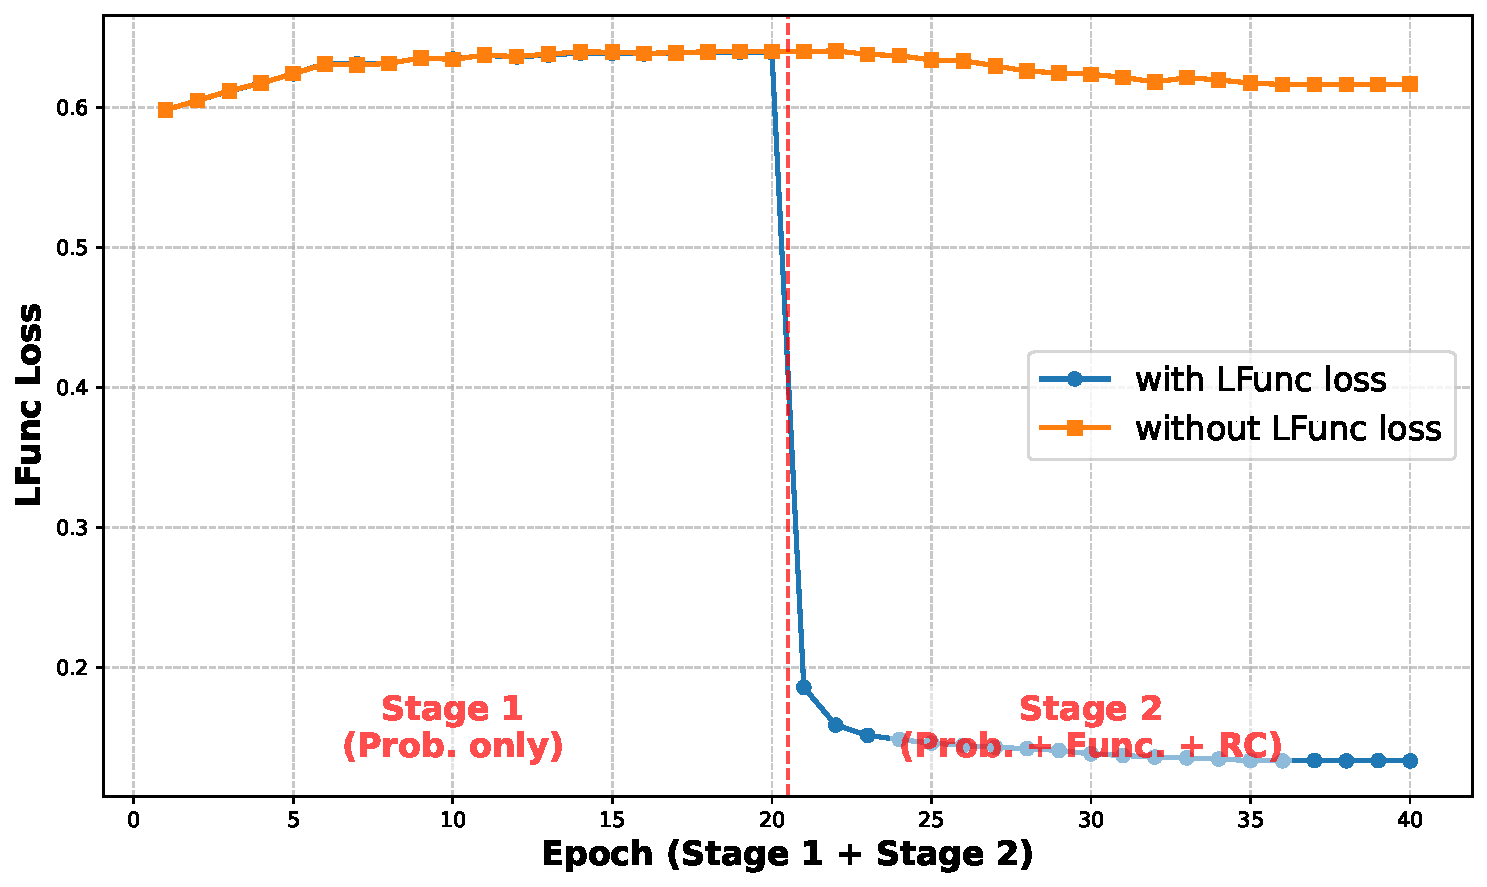
\includegraphics[width=0.7\linewidth]{no_tt_lfunc.pdf}
  \end{figure}
  
  \item 從 \autoref{fig:no_tt_lfunc} LFunc Loss 的學習曲線可以明顯觀察到，拔除 Pairwise TT Loss 的模型 (without LFunc loss) 在整個 Stage 2 的訓練過程中，其 LFunc 誤差始終維持在高點 (大於 0.6) 且幾乎沒有收斂跡象；相反地，Baseline 模型則迅速收斂至極低值。這顯示神經網路無法單憑訊號機率與電路結構特徵來隱式推導出邏輯閘的真值表差異，必須透過明確的 TT Loss 監督訊號才能有效學習。
  
  \begin{figure}[H]
    \centering
    \caption{開關 Pairwise TT Loss 之 Accuracy 比較}
    \label{fig:no_tt_accuracy}
    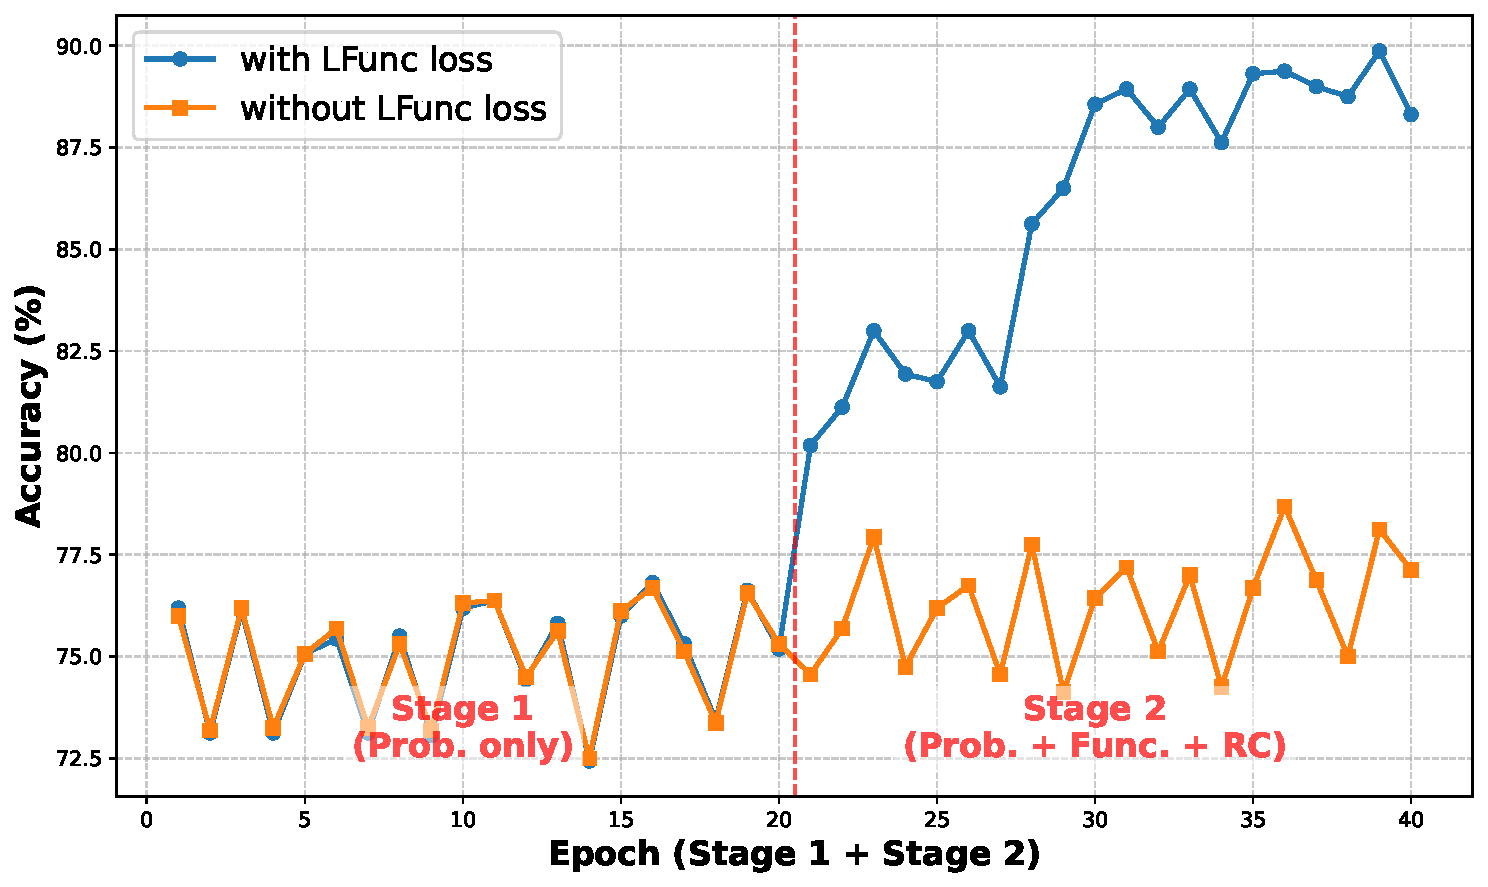
\includegraphics[width=0.7\linewidth]{no_tt_accuracy.pdf}
  \end{figure}
  
  \item 在 \autoref{fig:no_tt_accuracy} Accuracy 的表現上，兩者的差距更為顯著。Baseline 模型的準確率在 Stage 2 穩定攀升至接近 90\%；而沒有 LFunc loss 的模型則停滯在 75\% 至 78\% 之間劇烈震盪。這印證了 DeepGate2 所提出的 "NOT gate problem"：當缺乏 Pairwise TT Loss 時，模型會將機率特徵相似但邏輯功能完全相反的邏輯閘誤判為高度相似，導致嚴重的分類錯誤。因此，Pairwise TT Loss 是迫使模型學習邏輯閘真實功能、突破準確率瓶頸不可或缺的關鍵設計。
\end{itemize}

\subsection{Orthogonal PI Initialization 之有效性}

為了追蹤 Reconvergence 情況，DeepGate2 預設會給予每個 PI 一個獨一無二的正交向量作為初始特徵，如此訊號在某個節點分岔，於下游節點再次交會後，就能有效分辨訊號來自哪些 PI。

從 \texttt{src/models/mlpgate.py} 中的 \texttt{forward} 函數可以發現，只要在執行指令中加入 \texttt{--disable\_encode} 選項，就可以讓所有 PI 節點使用 homogeneous 的零向量 (\texttt{torch.zeros(num\_nodes, \\ self.dim\_hidden)})，而非正交向量 (\texttt{generate\_hs\_init}、\texttt{generate\_orthogonal\_vectors})。

\begin{figure}[H]
  \centering
  \caption{Orthogonal 與 Homogeneous 初始特徵之 LRC 比較}
  \label{fig:no_orthogonal_pi_lrc}
  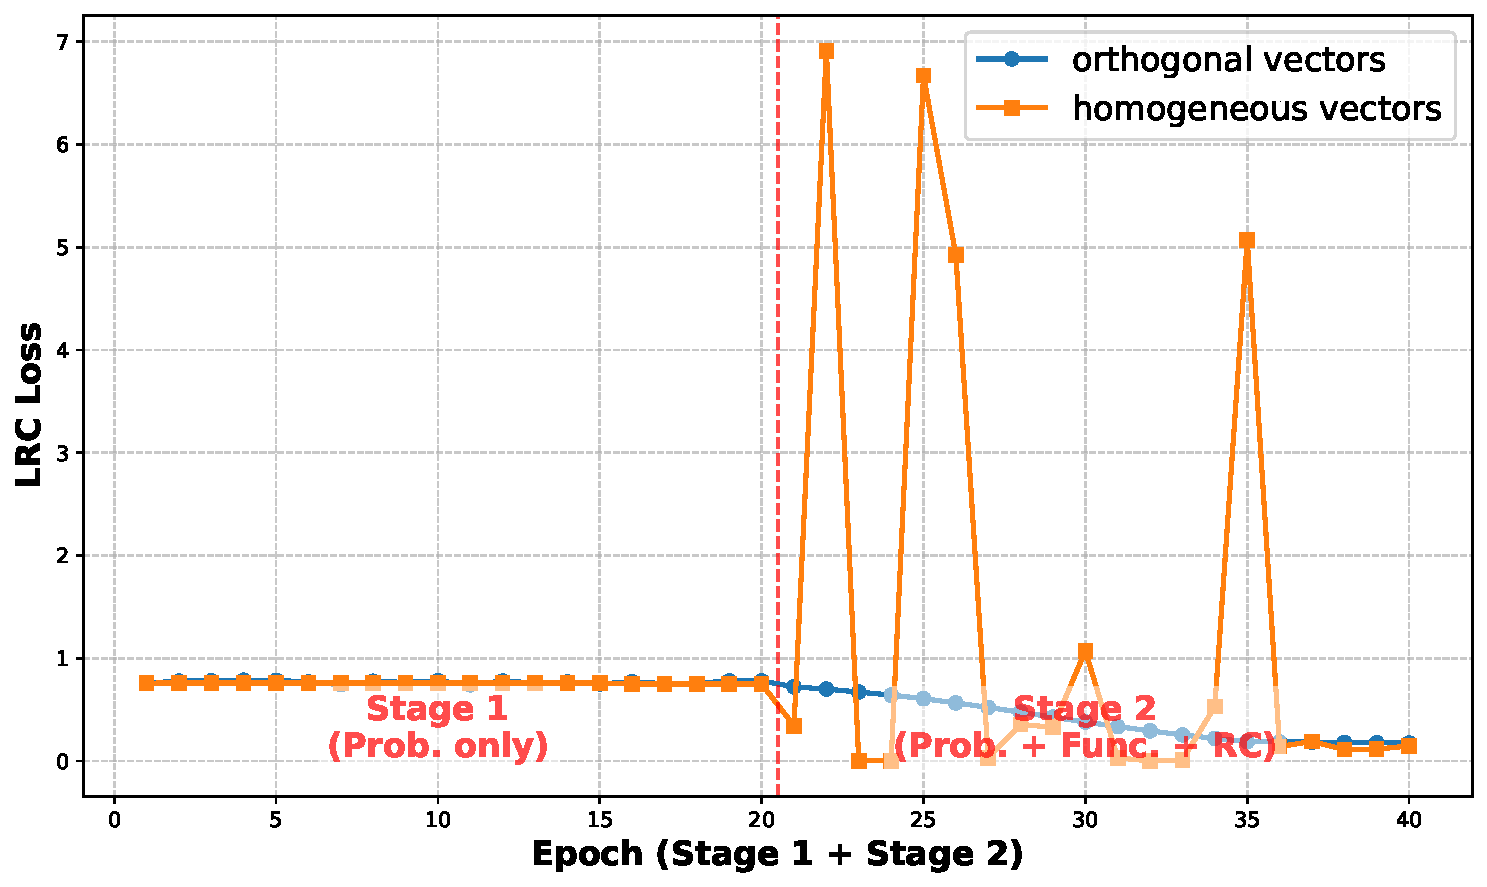
\includegraphics[width=0.7\linewidth]{no_orthogonal_pi_lrc.pdf}
\end{figure}

從 \autoref{fig:no_orthogonal_pi_lrc} LRC 中可以發現，拔除了 Orthogonal PI Initialization 的模型，在進入 Stage 2 後其 LRC Loss 出現了非常劇烈的震盪，完全無法收斂。相對而言，具備正交向量的 Baseline 模型則能保持在極低的誤差範圍。這項結果證明，若缺乏彼此獨立的正交初始特徵，神經網路根本無法有效進行 Reconvergence analysis。


\section{實驗結果位置}

上述所有實驗結果皆存放於 \href{https://github.com/co0okie/NTUST-Logic-Synthesis-and-Verification-PA2-DeepGate2/tree/main/exp/prob}{https://github.com/co0okie/NTUST-Logic-Synthesis-and-Verification-PA2-DeepGate2/tree/main/exp/prob} 上。

\end{document}